% APLAS 2021: Regular research papers should not exceed 18 pages in
% the Springer LNCS format(LaTeX template), including bibliography and
% figures.
% Lightweight double-blind: Author names and institutions must be
% omitted and References to the authors’ own related work should be in
% the third person 
%
\documentclass[runningheads]{llncs}
\pdfoutput=1
%\usepackage[english]{babel}
\usepackage[utf8]{inputenc}
\usepackage{amsmath}
\usepackage{amssymb}
%\usepackage{graphicx}
%\usepackage[colorinlistoftodos]{todonotes}
\usepackage{mathpartir}
\usepackage{graphicx}
%\usepackage{fixme}
\usepackage{xcolor}
\usepackage{hyperref}
\usepackage{listings}
\usepackage{titling}
\usepackage{pgfplots}
\pgfplotsset{compat=1.17}
\usepackage{tikz}
\usetikzlibrary{positioning}
\usepackage{amsmath}
\usetikzlibrary{shapes.geometric, arrows}
\usepackage{comment}
\usepackage{array}
\usepackage{booktabs}
\usepackage{hyperref}
\tikzstyle{startstop} = [rectangle, rounded corners, minimum width=3cm, minimum height=1cm,text centered, draw=black, fill=red!30]
\tikzstyle{process} = [rectangle, minimum width=3cm, minimum height=1cm, text centered, draw=black, fill=orange!30]
\tikzstyle{decision} = [diamond, minimum width=3cm, minimum height=1cm, text centered, draw=black, fill=blue!30]
\tikzstyle{arrow} = [thick,->,>=stealth]



%%% structure
\newcommand{\Angle}[1]{\langle#1\rangle}

%% values
\newcommand{\NEG}{\neg}
\newcommand{\CNF}{\wedge}
\newcommand{\DNF}{\vee}
\newcommand{\TRUE}{\text{True}}
\newcommand{\FALSE}{\text{False}}
\newcommand{\EMPTYSTRING}{\text{$""$}}
\newcommand{\STACKCONCAT}{\text{$::$}}
\newcommand{\ZERO}{\text{0}}
\newcommand{\ONE}{\text{1}}
\newcommand{\VAMOUNT}{\text{amount}}
\newcommand{\VCONTRACT}{\text{contract}}

%% contract constants
\newcommand{\CAMOUNT}{\text{amount}}
\newcommand{\CBALANCE}{\text{balance}}
\newcommand{\CSENDER}{\text{sender}}
\newcommand{\CSOURCE}{\text{source}}
\newcommand{\CNOW}{\text{now}}
\newcommand{\CLEVEL}{\text{level}}
\newcommand{\CCHAINID}{\text{chain-id}}
\newcommand{\CSELF}{\text{self}}
\newcommand{\CSELFADDRESS}{\text{self-address}}
\newcommand{\CTOTALVOTINGPOWER}{\text{total-voting-power}}
\newcommand{\CVOTINGPOWER}{\text{voting-power}}

%% contract instructions
\newcommand{\AMOUNT}{\text{AMOUNT}}
\newcommand{\BALANCE}{\text{BALANCE}}
\newcommand{\SENDER}{\text{SENDER}}
\newcommand{\SOURCE}{\text{SOURCE}}
\newcommand{\NOW}{\text{NOW}}
\newcommand{\LEVEL}{\text{LEVEL}}
\newcommand{\CHAINID}{\text{CHAIN-ID}}
\newcommand{\SELF}{\text{SELF}}
\newcommand{\SELFADDRESS}{\text{SELF-ADDRESS}}
\newcommand{\TOTALVOTINGPOWER}{\text{TOTAL-VOTING-POWER}}
\newcommand{\VOTINGPOWER}{\text{VOTING-POWER}}
\newcommand{\MinusBalanceAmount}{\text{BALANCE-AMOUNT}}
%% auction contract
\newcommand{\AuctionOwner}{\text{auction-owner}}
\newcommand{\AuctionBidder}{\text{auction-bidder}}
\newcommand{\AuctionClose}{\text{auction-close}}
\newcommand{\AuctionOpen}{\text{auction-open}}
\newcommand{\AuctionBid}{\text{auction-bid}}

%% system definition
\newcommand{\VAL}{\textbf{v}}
\newcommand{\VAR}{\textbf{x}}
\newcommand{\VARIABLE}{\text{$Var$}}
\newcommand{\CONSTANT}{\text{$Const$}}
\newcommand{\TERM}{\text{$T$}}
\newcommand{\VariableX}{\text{$x$}}
\newcommand{\VariableV}{\text{$v$}}
\newcommand{\VariableK}{\text{$k$}}
\newcommand{\VariableA}{\text{$a$}}
\newcommand{\VariableB}{\text{$b$}}
\newcommand{\ELT}{\text{$Elt$}}
\newcommand{\A}{\text{$A$}}
\newcommand{\B}{\text{$B$}}
\newcommand{\N}{\text{$n$}}
\newcommand{\K}{\text{$k$}}
\newcommand{\V}{\text{$v$}}
\newcommand{\M}{\text{$m$}}
\newcommand{\VariableOne}{\text{$x_1$}}
\newcommand{\VariableTwo}{\text{$x_2$}}
\newcommand{\VariableN}{\text{$x_n$}}
\newcommand{\Constant}{\text{$c$}}
\newcommand{\ConstantOne}{\text{$c_1$}}
\newcommand{\ConstantTwo}{\text{$c_2$}}
\newcommand{\ConstantN}{\text{$c_n$}}
\newcommand{\LIST}{\text{$l$}}
\newcommand{\EMPTYLIST}{\text{$\{\}$}}
\newcommand{\TLIST}{\text{$l'$}}
\newcommand{\HEAD}{\text{$hd$}}
\newcommand{\TAIL}{\text{$tl$}}
\newcommand{\STAIL}{\text{$< tl >$}}
\newcommand{\Term}{\text{$t$}}
\newcommand{\TermOne}{\text{$t_1$}}
\newcommand{\TermTwo}{\text{$t_2$}}
\newcommand{\TermN}{\text{$t_n$}}
\newcommand{\TermB}{\text{$t_b$}}
\newcommand{\STACK}{\text{$S$}}
\newcommand{\EMPTYSTACK}{\text{[ ]}}
\newcommand{\STACKONE}{\text{$S$}}
\newcommand{\STACKTWO}{\text{$S$}}
\newcommand{\STACKN}{\text{$S$}}
\newcommand{\Stack}{\text{$s$}}
\newcommand{\StackOne}{\text{$s_1$}}
\newcommand{\StackTwo}{\text{$s_2$}}
\newcommand{\StackN}{\text{$s_n$}}
\newcommand{\TSTACK}{\text{$S'$}}
\newcommand{\TStack}{\text{$s'$}}
\newcommand{\STATE}{\text{$ST$}}
\newcommand{\STATEONE}{\text{$ST_1$}}
\newcommand{\STATETWO}{\text{$ST_2$}}
\newcommand{\STATEN}{\text{$ST_n$}}
\newcommand{\SYSTEM}{\text{$SE$}}
\newcommand{\INSTRUCTION}{\text{$I$}}
\newcommand{\TINSTRUCTION}{\text{$I'$}}
\newcommand{\INSTRUCTIONONE}{\text{$I1$}}
\newcommand{\INSTRUCTIONTWO}{\text{$I2$}}
\newcommand{\Instruction}{\text{$i$}}
\newcommand{\TInstruction}{\text{$i'$}}
\newcommand{\InstructionOne}{\text{$i_1$}}
\newcommand{\InstructionTwo}{\text{$i_2$}}
\newcommand{\InstructionN}{\text{$i_n$}}
\newcommand{\Invariant}{\text{$Iv$}}
\newcommand{\PREDICATE}{\text{$P$}}
\newcommand{\PREDICATEA}{\text{$P_A$}}
\newcommand{\PREDICATEB}{\text{$P_B$}}
\newcommand{\Predicate}{\text{$p$}}
\newcommand{\Failwith}{\text{$Failwith$}}
\newcommand{\PredicateOne}{\text{$p_1$}}
\newcommand{\PredicateTwo}{\text{$p_2$}}
\newcommand{\PredicateN}{\text{$p_n$}}
\newcommand{\SETA}{\text{$\mathcal{A}$}}
\newcommand{\SETAAUCTION}{\text{$\mathcal{A}_{auction}$}}
\newcommand{\SETPOST}{\text{$\mathcal{A'}$}}
\newcommand{\SETPOSTAUCTION}{\text{$\mathcal{A'}_{auction}$}}
\newcommand{\EMPTY}{\text{$\O$}}
\newcommand{\PCreate}{\text{$P_{Create}$}}
\newcommand{\PBidding}{\text{$P_{Bidding}$}}
\newcommand{\PClose}{\text{$P_{Close}$}}
\newcommand{\SE}{\text{SE}}
\newcommand{\SINIT}{\text{$s_{init}$}}
\newcommand{\SFINAL}{\text{$s_{final}$}}
\newcommand{\FMAP}{\textbf{map}}
\newcommand{\MAPA}{\textbf{$map_A$}}
\newcommand{\MAPB}{\textbf{$map_B$}}
\newcommand{\MapBidding}{\textbf{$map_{bidding}$}}
\newcommand{\MapCreate}{\textbf{$map_{create}$}}
\newcommand{\MapClose}{\textbf{$map_{close}$}}
\newcommand{\MAPER}{\text{$\overline{\textbf{map}}$}}


%% operation
\newcommand{\CONS}{\text{cons}}
\newcommand{\NIL}{\text{nil}}
\newcommand{\PLUS}{\textbf{+}}
\newcommand{\MINUS}{\textbf{-}}
\newcommand{\EQUAL}{\textbf{=}}
\newcommand{\LESS}{\textbf{$<$}}
\newcommand{\LESSEQUAL}{\textbf{$<=$}}
\newcommand{\MORE}{\textbf{$>$}}
\newcommand{\MOREEQUAL}{\textbf{$>=$}}

%% instructions
\newcommand{\UNIT}{\text{Unit}}
\newcommand{\PAIR}{\text{Pair}}
\newcommand{\LEFT}{\text{Left}}
\newcommand{\RIGHT}{\text{Right}}
\newcommand{\SOME}{\text{Some}}
\newcommand{\NONE}{\text{None}}
\newcommand{\ADD}{\text{ADD}}
\newcommand{\DROP}{\text{DROP}}
\newcommand{\LOOP}{\text{LOOP}}
\newcommand{\FAILWITH}{\text{FAILWITH}}
\newcommand{\TRANSFER}[2]{\text{Transfer($#1$, $#2$)}}
\newcommand{\CONTRACT}{\text{CONTRACT}}
\newcommand{\CAR}{\text{CAR}}
\newcommand{\EXEC}{\text{EXEC}}
\newcommand{\APPLY}{\text{APPLY}}
\newcommand{\IF}{\text{IF}}
\newcommand{\IFLEFT}{\text{IF-LEFT}}
\newcommand{\IFRIGHT}{\text{IF-RIGHT}}
\newcommand{\IFCONS}{\text{IF-CONS}}
\newcommand{\ITER}{\text{ITER}}
\newcommand{\TITER}{\text{ITER'}}
\newcommand{\DIG}{\text{DIG}}
\newcommand{\DIP}{\text{DIP}}
\newcommand{\DIPN}{\text{DIP n}}
\newcommand{\TDIP}{\text{DIP'}}
\newcommand{\ABS}{\text{ABS}}
\newcommand{\COMPARE}{\text{COMPARE}}
\newcommand{\TCOMPARE}{\text{COMPARE'}}
\newcommand{\HASHKEY}{\text{HASH-KEY}}
\newcommand{\CONCAT}{\text{CONCAT}}
\newcommand{\TCONCAT}{\text{CONCAT'}}
\newcommand{\MEN}{\text{MEN}}
\newcommand{\TMEN}{\text{MEN'}}
\newcommand{\TMAP}{\text{MAP'}}
\newcommand{\PUSH}{\text{PUSH}}
\newcommand{\XOR}{\text{XOR}}
\newcommand{\MAP}{\textbf{MAP}}
\newcommand{\LAMBDA}{\text{LAMBDA}}


%symbols
\newcommand{\Overline}[1]{\text{$\overline{#1}$}}
\newcommand{\Mapsto}{\text{$\mapsto$}}
\newcommand{\Mid}{\text{$\mid$}}
\newcommand{\Mathcal}[1]{\text{$\mathcal{#1}$}}
\newcommand{\Models}{\text{$\models$}}
\newcommand{\SRightarrow}{\text{$\rightarrow$}}
\newcommand{\NSRightarrow}{\text{$\nrightarrow$}}
\newcommand{\Wedge}{\text{$\wedge$}}
\newcommand{\At}{\text{$@$}}
\newcommand{\Subseteq}{\text{$\subseteq$}}
\newcommand{\Vee}{\text{$\vee$}}
%\newcommand{\Cup}{\text{$\cup$}}
\newcommand{\STRINGCONCAT}{\text{$\hat{}$}}
\newcommand{\DOT}{\text{$...$}}


%% functions
\newcommand{\FABS}[1]{\text{abs($#1$)}}
\newcommand{\FXOR}{\text{xor}}
\newcommand{\FHASHKEY}[1]{\text{hash-key($#1$)}}
\newcommand{\FCONCAT}[1]{\text{concat($#1$)}}
\newcommand{\FGetTy}[1]{\text{get-ty($#1$)}}
\newcommand{\FLEN}[1]{\text{len($#1$)}}
\newcommand{\FAND}{\text{and}}
\newcommand{\FOR}{\text{or}}
\newcommand{\FNOT}{\text{not}}
\newcommand{\GETCONTRACTTYPE}{\text{get-contract-type}}
\newcommand{\UNOP}{\text{unop}}
\newcommand{\BINOP}{\text{binop}}



%% transition relations
\newcommand{\StateTrans}{\text{$\longrightarrow_S$}}
\newcommand{\ExprTrans}{\text{$\longrightarrow_E$}}
\newcommand{\SystemTrans}{\text{$\longrightarrow$}}


%% types
\newcommand\TEnv{\Gamma}
\newcommand\JTypeCode[2]{\vdash_C#1 : #2}
\newcommand\JTypeValue[2]{\vdash_V#1 : #2}
\newcommand\JTypeExpr[3]{#1 \vdash #2 : #3}
\newcommand{\TY}{\text{ty}}
\newcommand{\TYF}{\text{ty$_{1}$}}
\newcommand{\TYS}{\text{ty$_{2}$}}
\newcommand{\TYT}{\text{ty$_{3}$}}
\newcommand{\TYA}{\text{A}}
\newcommand{\TYB}{\text{B}}
\newcommand{\TYC}{\text{C}}
%% standard types
\newcommand{\TBOOL}{\text{bool}}
\newcommand{\TOR}{\text{or}}
\newcommand{\TYLIST}{\text{list}}
\newcommand{\TUNIT}{\text{unit}}
\newcommand{\TPAIR}{\text{pair}}
\newcommand{\TOPTION}{\text{option}}
\newcommand{\TMUTEZ}{\text{mutez}}
\newcommand{\TSTR}{\text{string}}
\newcommand{\TINT}{\text{int}}
\newcommand{\TNAT}{\text{nat}}
\newcommand{\TKEY}{\text{key}}
\newcommand{\TKEYHASH}{\text{key-hash}}
\newcommand{\TSIG}{\text{signature}}
\newcommand{\TADDR}{\text{address}}
\newcommand{\TTIME}{\text{timestamp}}
\newcommand{\TCONTRACT}{\text{contract}}
\newcommand{\TCHAINID}{\text{chain-id}}
\newcommand{\TLAMBDA}{\text{lambda}}







%% typing related
\newcommand{\EmptyEnv}{\cdot}

%% evaluation contexts
\newcommand\EC[1]{\epsilon[#1]}

%% metavariables


%%% Local Variables:
%%% mode: latex
%%% TeX-master: "paper"
%%% End:

%
%------------------------------------------------------------------------------
%       package includes
%------------------------------------------------------------------------------
    % font encoding is set up for pdflatex, for other environments see
    % http://tex.stackexchange.com/questions/44694/fontenc-vs-inputenc
    \usepackage[T1]{fontenc}  % 8-bit fonts, improves handling of hyphenations
    \usepackage{lmodern}
    \usepackage[utf8x]{inputenc}
    % provides `old' commands for table of contents. Eases the ability to switch
    % between book and scrbook
    % cross-referencing
    \usepackage{xr}


    % ------------------- layout, default -------------------
    % adjust the style of float's captions, separated from text to improve readabilty
    \usepackage[labelfont=bf, labelsep=colon, format=hang, textfont=singlespacing]{caption}
    % With format = hang your caption will look like this:
    % Figure 1: Lorem ipsum dolor sit amet,
    %           consectetuer adipiscing elit.
    %           Ut purus elit, vestibulum
    % If you instead want
    % Figure 1: Lorem ipsum dolor sit amet,
    % consectetuer adipiscing elit. Ut purus
    % elit, vestibulum
    % change to format=plain
    \usepackage{chngcntr}  % continuous numbering of figures/tables over chapters
    \counterwithout{equation}{chapter}
    \counterwithout{figure}{chapter}
    \counterwithout{table}{chapter}

    % Uncomment the following line if you switch from scrbook to book
    % and comment the setkomafont line
    \usepackage{titlesec}  % remove "Chapter" from the chapter title
    \titleformat{\chapter}[hang]{\bfseries\huge}{\thechapter}{2pc}{\huge}
    % \setkomafont{chapter}{\normalfont\bfseries\huge}

    \usepackage{setspace}  % Line spacing
    \onehalfspacing
    % \doublespacing  % uncomment for double spacing, e.g. for annotations in correction

    % ------------------- functional, default-------------------
    \usepackage{natbib}
    \usepackage[dvipsnames]{xcolor}  % more colors
    \usepackage{array}  % custom format per column in table - needed on the title page
    \usepackage{graphicx}  % include graphics
    \usepackage{subfig}  % divide figure, e.g. 1(a), 1(b)...
    \usepackage{amsmath}  % |
    \usepackage{amsthm}   % | math, bmatrix etc
    \usepackage{amsfonts} % |
    \usepackage{calc}  % calculate within LaTeX
    \usepackage[unicode=true,bookmarks=true,bookmarksnumbered=true,
                bookmarksopen=true,bookmarksopenlevel=1,breaklinks=false,
                pdfborder={0 0 0},backref=false,colorlinks=false]{hyperref}
	\usepackage{listings}
	\usepackage{tabularx}
	\usepackage{makecell}
	\usepackage{upquote}

    %==========================================
    % You might not need the following packages, I only included them as they
    % are needed for the example floats
    % ------------------- functional, custom -------------------
    \usepackage{algorithm,algpseudocode}
    \usepackage{bm}  % bold greek variables (boldmath)
    \usepackage{tikz}
    \usetikzlibrary{positioning}  % use: above left of, etc

    % Improves general appearance of the text
    \usepackage[protrusion=true,expansion=true, kerning]{microtype}
    \usepackage{enumitem}

	\usepackage{csquotes}
	\usepackage{scrhack}

%------------------------------------------------------------------------------
%       (re)new commands / settings
%------------------------------------------------------------------------------
    % ----------------- referencing ----------------
    \newcommand{\secref}[1]{Section~\ref{#1}}
    \newcommand{\chapref}[1]{Chapter~\ref{#1}}
    \renewcommand{\eqref}[1]{Equation~(\ref{#1})}
    \newcommand{\figref}[1]{Figure~\ref{#1}}
    \newcommand{\tabref}[1]{Table~\ref{#1}}
    \newcommand{\lstref}[1]{Listing~\ref{#1}}
    %\newcommand{\algref}[1]{Algorithm~\ref{#1}}
    \newcommand*{\captionsource}[2]{%
  		\caption[{#1}]{%
    	#1%
    	\\\hspace{\linewidth}%
    	Source: #2%
  		}%
	}

    % ------------------- colors -------------------
    \definecolor{darkgreen}{rgb}{0.0, 0.5, 0.0}
    % Colors of the Albert Ludwigs University as in
    % https://www.zuv.uni-freiburg.de/service/cd/cd-manual/farbwelt
    \definecolor{UniBlue}{RGB}{0, 74, 153}
    \definecolor{UniRed}{RGB}{193, 0, 42}
    \definecolor{UniGrey}{RGB}{154, 155, 156}
    \definecolor{cverbbg}{gray}{0.93}

    % ------------------- layout -------------------
    % prevents floating objects from being placed ahead of their section
    \let\mySection\section\renewcommand{\section}{\suppressfloats[t]\mySection}
    \let\mySubSection\subsection\renewcommand{\subsection}{\suppressfloats[t]\mySubSection}


    % ------------------- marker commands -------------------
    % ToDo command
    \newcommand{\todo}[1]{\textbf{\textcolor{red}{(TODO: #1)}}}
    \newcommand{\extend}[1]{\textbf{\textcolor{darkgreen}{(EXTEND: #1)}}}
    % Lighter color to note down quick drafts
    \newcommand{\draft}[1]{\textbf{\textcolor{NavyBlue}{(DRAFT: #1)}}}
    \newcommand{\move}[1]{\textbf{\textcolor{Orange}{(MOVE?: #1)}}}


    % ------------------- math formatting commands -------------------
    % define vectors to be bold instead of using an arrow
    \renewcommand{\vec}[1]{\mathbf{#1}}
    \newcommand{\mat}[1]{\mathbf{#1}}
    % tag equation with name
    \newcommand{\eqname}[1]{\tag*{#1}}


    % ------------------- pdf settings -------------------
    % ADAPT THIS
    \hypersetup{pdftitle={\thetitle},
                pdfauthor={\theauthor},
                pdfsubject={Master's thesis at the Albert Ludwig University of Freiburg},
                pdfkeywords={blockchain, smart contract},
                pdfpagelayout=OneColumn, pdfnewwindow=true, pdfstartview=XYZ, plainpages=false}


    %==========================================
    % You might not need the following commands, I only included them as they
    % are needed for the example floats

    % ------------------- Tikz styles -------------------
    \tikzset{>=latex}  % arrow style


    % ------------------- algorithm ---------------------
    % Command to align comments in algorithm
    \newcommand{\alignedComment}[1]{\Comment{\parbox[t]{.35\linewidth}{#1}}}
    % define a foreach command in algorithms
    \algnewcommand\algorithmicforeach{\textbf{foreach}}
    \algdef{S}[FOR]{ForEach}[1]{\algorithmicforeach\ #1\ \algorithmicdo}

    % line spacing should be 1.5
    \renewcommand{\baselinestretch}{1.5}

    % set distance between items in a list, for more details see the
    % enumitem package: https://www.ctan.org/pkg/enumitem
    \setlist{itemsep=.5em}


% ------------------- colors -------------------
\definecolor{darkgreen}{rgb}{0.0, 0.5, 0.0}
\definecolor{UniBlue}{RGB}{0, 74, 153}
\definecolor{UniRed}{RGB}{193, 0, 42}
\definecolor{UniGrey}{RGB}{154, 155, 156}
\definecolor{cverbbg}{gray}{0.93}

\newcommand{\todo}[1]{\textbf{\textcolor{red}{(TODO: #1)}}}

\begin{document}
%
\title{Assertion Contracts}
%
%\titlerunning{Abbreviated paper title}
% If the paper title is too long for the running head, you can set
% an abbreviated paper title here
%
\author{Thi Thu Ha Doan\orcidID{0000-0001-7524-4497}\and Peter Thiemann\orcidID{0000-0002-9000-1239}}

%
%\authorrunning{Ha Doan, P. Thiemann}
% First names are abbreviated in the running head.
% If there are more than two authors, 'et al.' is used.
%
%\institute{University of Freiburg, Germany \\ \email{\{doanha,thiemann\}@informatik.uni-freiburg.de}
%}
%
\maketitle              % typeset the header of the contribution
%
\begin{abstract}
In certain blockchain scenarios, verifying properties of a parameter requires significant gas costs or may even be infeasible due to gas limits. This study proposes a distributed verification protocol to address this issue. The core idea is to distribute the negation of the assertion of a property to validators, who then attempt to find a counterexample off-chain. If a counterexample is found, it can be submitted and verified on-chain. Additionally, a proof-of-work-based incentive mechanism is proposed to encourage validators to participate in the distributed verification process.

To operationalize these ideas, we suggest a practical model that addresses potential security concerns. We  implemented a prototype of the proposed protocol and conducted a cost analysis to demonstrate the advantages of our method in terms of cryptocurrency, proving its practical utility.
 \keywords{}
\end{abstract}
%
%
%
\section{Introduction}
\label{sec:introduction}
Considering the example where a parameter $p$ is a prime number, the assertion in predicate logic for the parameter is:
\begin{gather}\label{eq:3a}
  (\forall n) (2 \le n \le \sqrt p) \Rightarrow (p \mathbin{\%} n) \ne 0
\end{gather}


\noindent and its negation form is 

\begin{gather}\label{eq:3b}
  (\exists n) (2 \le n \le \sqrt p) \wedge (p \mathbin{\%} n) = 0
\end{gather}

Each validator try to find  a
random $n$ in the range $2 \le n \le 
\sqrt p$ such that $(p \mathbin{\%} n) = 0$. If the remainder is $0$, the validator found a counterexample.

An other example, consider a contract that takes a sorted array of integers.
\begin{lstlisting}[numbers=none]
contract Sorted {
  function find (int[50] a, int v) public {
    // assume a is sorted
  }
}
\end{lstlisting}
The explicit assertion would be
\begin{gather}\label{eq:1a}
  (\forall k) (0\le k <49) \Rightarrow a[k] \le a[k+1]
\end{gather}
While we can check this contract in $O(1)$ time, the constant factor is big! So we
consider its negation.
\begin{displaymath}
  (\exists k) (0\le k <49) \wedge a[k] > a[k+1]
\end{displaymath}
Each validator attempts to find the number $k$ such that the negation is true for such $k$, then the validator has found a counterexample for the sortedness of the array.
\section{Primaries}
\label{sec:primaries}


\section{On-chain Assertions Verification}
\label{sec:assertion-verification-onchain}
\subsection{Problem}

In the context of a domain $A$ and a predicate $P$ on $A$, an assertion is formalized using the universal quantifier as follows:
\begin{gather}
  \label{eq:1b}
\forall a \in A. P_{a}
\end{gather}

This formula can be extended to multiple domains as:

\begin{gather}
\label{eq:2}
\forall a \in A, \forall b \in B, \dots .P_{a, b, \dots}
\end{gather} 

It requires iterating over the domain \( A \) within the contract to verify these assertions:
\begin{gather}
  \label{eq:3}
  \bigwedge_{a \in A} P(a)
\end{gather}

For multiple domains, the verification process can be expressed as:
\begin{gather}
  \label{eq:4}
  \bigwedge_{a \in A} \bigwedge_{b \in B} \dots P(a, b, \dots)
\end{gather}

When the domain $A$ is large or the predicate $P$ is complex to evaluate, it incurs a significant amount of gas to perform the verification process on-chain.  Given the current high gas prices, this could result in substantial costs or even impossible due to gas limits. 
\subsection{Use Cases}

\section{Distributed Assertions Verification}
\label{sec:distributed-assertion-verification}
\subsection{Off-chain Distributed Verification Approach}
We propose a novel approach for verifying parameter assertions in smart contracts on the blockchain. Our approach distributes the assertion verification process and moves it off-chain, with only the verification results being submitted to the blockchain.

Assertions are checked off-chain, and only the results of these checks (indicating whether any assertion was violated) are submitted and re-verified to the blockchain. This reduces the computational load on the blockchain while ensuring the integrity of the contract.

The outline of our approach is as follows:
\begin{enumerate}
\item Determinte the negation fomular of an assertion: The negation of the assertion \ref{eq:3} is represented by the existential quantifier formulas:

\begin{gather}
\label{eq:5}
\neg \left( \bigwedge_{a \in A} P(a) \right) \equiv \exists a \in A. \neg P(a)
\end{gather}

And for multiple domains \ref{eq:4}, it is as follows:

\begin{gather}
\label{eq:6}
\neg \left( \bigwedge_{a \in A} \bigwedge_{b \in B} \dots P(a, b, \dots) \right) \equiv \exists a \in A, \exists b \in B, \dots . \neg P(a, b, \dots)
\end{gather}
\item Off-chain verification: Validators endeavor to find counterexamples of the assertion using this negation off-chain. Specifically, each validator attempts to find a counterexample by identifying $a \in A$ such that the negation formula is satisfied $\neg P(a)$. 
\item On-chain re-verification: When a counterexample is found, the validator submits it, which is then re-verified on-chain. 
\end{enumerate}

Our approach aims to alleviate the expensive gas comsuming. Instead of verifying the entire assertion, the on-chain contract only needs to check specific points. Since only some specific points are checked on-chain, the amount of gas required for the computation to check the counterexample is likely to be significantly less than verifying the entire assertion directly on-chain.
\subsection{Proof-of-Work-Based Incentivization Mechanism}
Finding a counterexample is rewarded, incentivizing validators but at the cost of computing resources. Instances of finding a counterexample may be rare, as callers typically avoid passing invalid parameters into the blockchain. If no counterexample emerges, the verification accuracy depends on the number of attempts to negate the assertion, with more validators increasing the certainty. Therefore, it is crucial to encourage validators to engage in the verification process even without discovering a counterexample. %It is necessary to incentivize this effort. %Moreover, it is logical to reward only a portion of the computational effort required. 
%However, to prioritize the discovery of counterexamples, the reward for finding a counterexample is set significantly higher than that for providing a computational proof.

We propose a proof-of-work-based incentivization mechanism where validators are rewarded for discovering counterexamples, and others are rewarded for their computational efforts. This approach encourages participation in the distributed verification process, ensuring thorough validation even without the discovery of counterexamples.

A significant concern arises regarding how to recheck the counterexample and a computation efforts on-chain and ensure that validators perform the verification computation off-chain if no counterexample is found.
\subsubsection{Outlines}
Our proposed proof-of-work-based incentivization mechanism is outlined as follows:
\begin{itemize}
\item The counterexample is submitted in the form of the indication of the element where the assertion is invalid.
\item To prioritize the discovery of counterexamples, the reward for finding a counterexample is set significantly higher than that for providing a computational proof.
\item We utilize the proof-of-work concept by introducing a target hash \( t \) that sets the required difficulty level to earn the computation reward.
\item The objective of the validator is to find a counterexample or a computation proof that is smaller than or equal to the target hash \( t \).
\item The computation of the negation formula is integrated into a computational proof to ensure that the validators cannot produce the proof without executing a negation check.
\end{itemize}
%Because the rewards may be limited in quantity, validators are motivated to swiftly verify the parameters to claim the reward before others do so. 
\subsubsection{Reward computation}
The next question is how to devise a computational proof to incentivize computational effort. The key challenge is how to involve the negation check in the computational proof and how to reproduce the computational proof off-chain to on-chain with a reasonable gas cost. To address this, we introduce a seed $s$ in each verification process.

Let \( n \) denote the size of the domain \( A \). 
\begin{align}
n = |A|
\end{align}
where $\mid A \mid$ denotes the number of elements in the domain $A$.

Each number \( i \) in the range \([1, n]\) corresponds to an element in \( A \). 
\begin{align}
a=A[i]
\end{align}
where $A[i]$ denotes the $i$-th element in $A$.

The seed \( s \) is a random number, and we can reduce it modulo \( n \) to obtain \( i \), which is associated with an element \( a \) in \( A \).
\begin{align}
i = (s \mod n) + 1
\end{align}

\paragraph{Estimate the number of seeds:} We first estimate the number of seeds needed to find a counterexample with a given expected probability. %, assuming the worst case where only one validator participates.

Let's assume the unsatisfied element is only at the first element $a_0$ in $A$, and the number of seeds is $m$. Each seed independently has a probability of $1/n$ to detect the problem and a probability of $\frac{n-1}{n}$ not to detect the problem. Hence, if we assume that each seed associated with an element $a$ in $A$ is chosen independently from a uniform distribution, the probability that no seed checks the element $a_0$ converges to $0$ as the number of seeds approaches infinity:

\[
  \lim_{m \to \infty} \frac{(n-1)^m}{n^m} = \lim_{m \to \infty} \left( \frac{n-1}{n} \right)^m = 0
\]

Depending on the expected probability to detect the problem, the number of seeds to generate can be determined. 

Assume that $p$ is the probability of finding at least one counterexample. The complementary probability is used to calculate the number of seeds $m$ needed to achieve a given expected probability $p$ of finding a counterexample.
\begin{itemize}
\item The probability of a single seed failing to find a counterexample is $\frac{n-1}{n}$.
\item The probability of all $m$ seeds failing to find a counterexample is $\left(\frac{n-1}{n}\right)^m$.
\item The probability of at least one of the $m$ seeds finding a counterexample is:
\[
p = 1 - \left(\frac{n-1}{n}\right)^m
\]
\end{itemize}  

Rearranging to solve for \( m \):

\[
\left(\frac{n-1}{n}\right)^m = 1 - p
\]

Taking the natural logarithm on both sides:

\[
\ln\left(\left(\frac{n-1}{n}\right)^m\right) = \ln(1 - p)
\]

\[
m \ln\left(\frac{n-1}{n}\right) = \ln(1 - p)
\]

Solving for \( m \):

\[
m = \frac{\ln(1 - p)}{\ln\left(\frac{n-1}{n}\right)}
\]

Note that $p$ is the probability obtained when only one validator participates in the verification process. As more validators become involved, the probability of discovering a counterexample increases.
\paragraph{Set up the taget hash:}
The above number of seed $m$ can then be used to set up the target hash $t$. The target hash $t$ can be calculated based on a desired difficulty level. In proof-of-work systems, difficulty is typically adjusted to ensure that the average efforts to find a valid hash. The target hash $t$ is often calculated by taking the maximum possible hash value and dividing it by the difficulty level:
\[
t = \frac{H_{\text{max}}}{D}
\]

Where:
\begin{itemize}
  \item \( H_{\text{max}} \) is the maximum possible hash value.
  \item \( D \) is the difficulty level, which can be adjusted based on the expected number of trials.
\end{itemize}


Given the expected number of seeds to generate, 
the difficulty level $D$ can be adjusted accordingly. Typically, $D$ is set to ensure that a valid hash is found approximately once every $m$ trials.

If we want the probality of finding a valid hash to be $\frac{1}{m}$, then:
\[
D=m
\]

For a 256-bit hash, $H_{\text{max}}$ is $2^{256} - 1 $.  using the maximum hash value and the difficulty level, the target hash $t$ is:
    
\[
\frac{2^{256} - 1}{m}
\]
\paragraph{Conduct a computation hash:} The computation of the negation formula is integrated into a computational proof to ensure that the validators cannot produce the proof without executing a negation check.

Lets \(\text{eval}\) be the function that returns the significant components of the evaluation of the negation \(\neg P(a)\).  For example, it returns \(a[i]\) and \(a[i + 1]\) in the evaluation of the negation predicate \(a[i] < a[i+1]\) in the sorted array example.

Thus, the computation hash includes the seed  \( s \) and \(\text{eval}\). 
\begin{align}
t_s = \text{hash}(s, \text{eval}(\neg P(a)))
\end{align}
\subsubsection{On-chain re-verification}
Given a submitted seed $s$: 
\begin{align}
s \in \mathbb{N} 
\end{align}
where $s$ is a random natural number.

The on-chain contract will recompute to determine whether the submitted seed produces a counterexample, qualifies for a computation reward, or does not qualify for a reward. The rechecking process is as follows:
\begin{enumerate}
\item Calculate $n$ as the size of the domain $A$.
\item Determine the tagert $t$.
\item Calculate $i \in [1, n]$ based on $s$ using the modulo operation.
\item Associate \( i \) with the corresponding element $a$ in $A$.
\item Perform the negation check $\neg P(a)$ to detect a counterexample if any.
\item If no counterexample is found, calculate the hash \( t_s \) corresponding to the seed \( s \).
\item Compare \( t_s \) to the target hash to determin whether it is a reward computation.
\end{enumerate}

After conducting the negation check, either a counterexample is identified, or a hash is computed based on the seed $s$ along with the evaluation of the condition $\neg P_{a}$. This hash is then compared with the target hash to ascertain if it meets the criteria for a reward computation. The outcomes of the verification process include either a counterexample, a reward computation, or a non-reward computation.
\subsubsection{Off-chain verification}
In order to win a reward, either for discovering a counterexample or providing a computation proof, a validator must run the negation check off-chain. Due to the setup of the target hash, a validator needs to generate approximately $m$ seeds to have a chance of discovering a counterexample or a computation proof, thereby ensuring the validity or revealing the invalidity of a parameter.

The sequence of operations to find a seed can be described in Fig. \ref{fig:find_seed}. During the distributed process, each validator may generate a seed $s$ and conducts the negation check until the outcome indicates either a counterexample or a reward computation. Upon achieving either of these outcomes, the validator is able to submit it on-chain to claim their reward. 

Both the counterexample and the computation proof are represented by the seed used, allowing the on-chain compoment to replicate the process to verify its validity. If the verification is successful, the validators will be entitled to receive their reward.

\begin{figure}
    \centering
\begin{tikzpicture}[node distance=2cm]
    % Nodes
    \node (calc_n) [process] {$n = |A|$};
    \node (start) [startstop, below of=calc_n] {$s$};
    \node (calc_i) [process, below of=start] {$i = (s \mod n) + 1$};
    \node (find_a) [process, below of=calc_i] {$a = A[i]$};
    \node (counterexample) [decision, below of=find_a, yshift=-0.5cm] {$\neg P(a)$};
    \node (calc_hash) [process, below of=counterexample, yshift=-0.5cm] {$t_s = \text{hash}(s, \text{eval}(\neg P(a)))$};
    \node (compare) [decision, below of=calc_hash, yshift=-0.5cm] {$t_s <= t$};
    \node (submit) [startstop, below of=compare, yshift=-0.5cm] {Submit on-chain};
    % Arrows
    \draw [arrow] (calc_n) -- (start);
    \draw [arrow] (start) -- (calc_i);
    \draw [arrow] (calc_i) -- (find_a);
    \draw [arrow] (find_a) -- (counterexample);
    \draw [arrow] (counterexample) -- node[midway, above, sloped, anchor=center, yshift=0.5em] {No} (calc_hash);
    \draw [arrow] (calc_hash) -- (compare);
    %\draw [arrow] (compare) -- node[anchor=south] {Yes} (submit);
    \draw [arrow] (compare) -- (submit) node[midway, above, sloped, anchor=center, yshift=0.5em] {Yes};
    % Right-angle arrow from counterexample to submit
	\draw [arrow] (counterexample.east) -| node[pos=0.25, above] {Yes} ([xshift=2cm]submit.east) |- (submit);
	\draw [arrow] (compare.west) -| node[pos=0.75, left] {No} ([xshift=-2cm]counterexample.west) |- (start);
\end{tikzpicture}
\caption{Finding a reward seed.}
\label{fig:find_seed}
\end{figure}

%Consequently, each seed $s$ is linked with an element $a$ in the domain $A$, followed by the evaluation of the negation of the assertion $\neg P_{a}$. 

 

%The next question is associte a seed with an elemnt in the domain. Let $n$ be the size of the domain $A$.  We'll consider two cases: (1) when it is straightforward to associate a natural number $i$ to an element of $A$, such as a natural number, integer, or array, and (2) when it is not.

%In the first case, the seed $s$ is a random number. It is then modulated with the size $n$ to obtain $i$, which is then associated with an element $a$ in $A$. 

%\begin{gather}\label{}
%i = s \mod n
%\end{gather}



%In the second case, when it is not straightforward to associate a natural number with an element of the domain, then the seed is limited to the elements of the domain. The concern in this case is that the target $t$ needs to be set up in such a way that there is a guarantee to possibly find a reward computation.

%Let's examine an assertion in smart contract languages such as Solidity and Michelson. An assertion is essentially a predicate logic expressed as a boolean formula computed from relational operators ($=$, $!=$, $>$, $<$, $>=$, $<=$), logical operators ($!$, $\&\&$, $\|$), and expressions. Let $\pi_{P_{a}}$ = {$e_1$, $e_2$, \dots } represent the set of expressions involved in the computation of the predicate $P_a$. The hash of the seed and these expressions ($s$, $\pi_{P_{a}}$) is then computed and compared with the target hash. Since the hash involves $\pi_{P_{a}}$, the validator needs to execute the condition check to find a reward computation.


\section{Practical model}
\subsection{Security risks}
Distributed verification of assertions is indeed an intriguing concept, yet it faces the following security risks when proposing an incentive method:

\begin{enumerate}
\item Front-running attacks: The system is vulnerable to front-running attacks, where an attacker closely monitors the mempool to intercept a seed representing a counterexample or a computation proof, subsequently stealing the reward.
\item Caller exploitation: A caller might exploit the system by running the negation check privately to identify the reward before submitting the parameter on-chain, thereby swiftly claiming the reward ahead of the other validators. 
\item Denial-of-service (DoS) attacks: The system is susceptible to DoS attacks, where a caller inundates the system with numerous invalid parameters, causing congestion and hindering its operation.
%\item Reward manipulation: A validator may attempt to manipulate the reward system by resubmitting counterexamples or computation proofs multiple times to multiply their rewards.
\end{enumerate}
\subsection{Overview architect}
This section presents a practical model that unifies theoretical principles and addresses the previously mentioned security concerns. The architectural design of this model is depicted in Figure \ref{fig.architect}. The model consists of two main entities: the on-chain assertion contract and the off-chain validator program. 
\paragraph{Main actors.} Three distinct actors play key roles.
\begin{itemize}
\item Owner: responsible for deploying and overseeing both on-chain and off-chain components.
\item Callers: engage with on-chain contracts by initiating assertions and interacting with the system.
\item Validators: tasked with validating parameters and ensuring the integrity of the verification process.
\end{itemize}
\paragraph{On-chain assertion contract.}
While additional functions may exist, the assertion contract must encompass the following two essential functions:
\begin{itemize}
\item The \lstinline|submit_parameter| function: Callers utilize this function to submit their parameters for validation. Subsequently, the parameter is distributedly verified by validators.
\item  The \lstinline|claim_reward| function: This function accepts a parameter and a seed as inputs, yielding a result indicating whether the computation from the seed results in a counterexample, a reward computation, or a non-reward computation.
\end{itemize}
\paragraph{Off-chain assertion contract.}
Since the off-chain contract runs off-chain, it can be implemented according to the validator's preferences. However, the crucial point is that the off-chain contract must use the exact same \lstinline|claim_reward| function when attempting to find a counterexample or a computation proof. Additionally, it should support a function that assists the validator in finding a seed to earn a reward.
\paragraph{Storage.}
When a parameter is submitted for verification, the following information should be stored:
\begin{itemize}
\item Parameter: this includes the parameter itself. In cases where storing the parameter on-chain is impractical because of its size, it could be possible to store only its hash. Despite this, the hash remains sufficient for validation.
\item Timestamp: this indicates the approximate time when the parameter was submitted. This information is used to prevent caller exploitation security risks as explained above.
\end{itemize}

In some applications, multiple computational proofs may be allowed. There are a record to monitor the progress of the parameter's verification. This record is crucial for determining when a work function can be invoked for a given parameter or when it should be discarded. The verification status records a counterexample and reward computations found. For that, it should include the following details of the addresses of the validators and the random number $r$ used in the verification process.
\begin{figure}
\centering
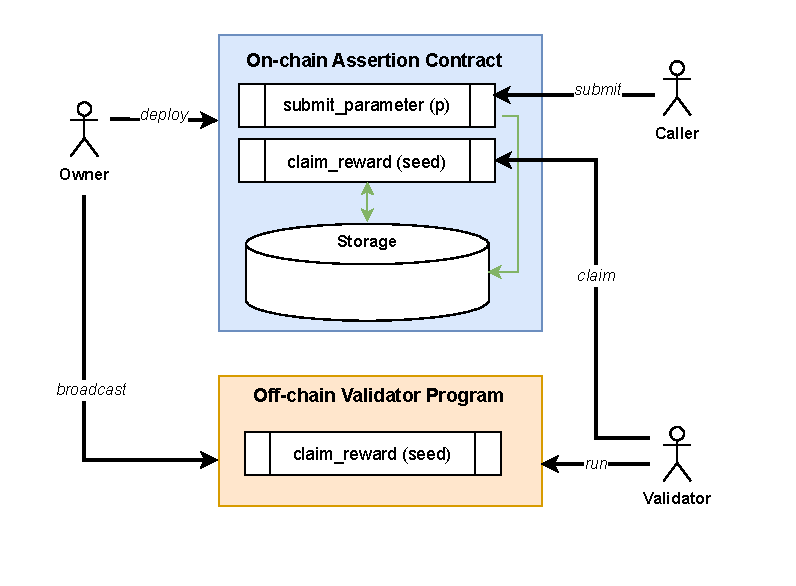
\includegraphics[scale=.8]{assertion}
\caption{The architecture of the practical model}
\label{fig.architect}
\end{figure}




\subsubsection{Calculate seed.}
While a random number alone is sufficient to indicate the associated element $a$ in the domain $A$, to prevent the front-running attack and the caller exploitation attack, we enhance the randomness of the seed by combining a random number with the validator's address and the timestamps indicating when the parameter is submitted on the chain to calculate the seed. In deeds, the validator's address and timestamps are converted to numerical values and use these numbers in combination with a random number to compute the seed. This combination adds an extra level of security. 
\begin{enumerate}
\item 
Seed calculation: The seed is enhanced by combining a random number with the validator's address and timestamps. Let's denote the random number by $r$, the validator's address by $addr$, and the timestamp by $t$.
\begin{equation}
r \in \mathbb{N}, \quad \text{addr} \in \text{Addresses}, \quad t \in \text{Timestamps}
\end{equation}
\item Conversion of address and timestamp: The address and timestamp are converted to numerical values using appropriate functions.
\begin{equation}
\text{addr\_num} = \text{init256}(\text{addr}) \\
 \quad t_{\text{num}} = \text{convert}(t)
\end{equation}
\item Combination to compute the seed: The seed $s$ is computed by combining these numerical values.
\begin{equation}
s = \text{hash}(r, \text{addr\_num}, t_{\text{num}})
\end{equation}
where \(\text{hash}\) is a hash function that takes the three numerical values and returns a numerical value \( s \).
\end{enumerate}

\textbf{Security Features}:
\begin{itemize}
    \item Front-running attacks: Other validators cannot use the random number $r$ alone because the combination with their address and timestamp will not produce the same seed $s$.
    \item Caller exploitation: The timestamp constraints prevent the caller from running the check before submitting the parameter.
\end{itemize}
%In this system, even if other validators obtain a random number, they are unable to submit it successfully, as their combination with their address will not yield the correct seed that corresponds to a specific element in the domain. Additionally, a caller cannot run the check before submitting the parameter owing to the timestamp constraints. 
As a result, any attempt to submit manipulated or before-run seeds will fail to produce either a counterexample or reward computation. The address conversion can be achieved using functions such as \lstinline|init256| in Solidity, which transform an Ethereum address into a numerical value. 

\subsubsection{The evaluation of the negation predicate.} An assertion in smart contract languages, such as Solidity and Michelson, is essentially predicate logic expressed as a Boolean formula computed from relational operators, logical operators, and expressions. 
\begin{align}
\text{Relational operators: } & =, \neq, >, <, \geq, \leq \\
\text{Logical operators: } & \neg, \land, \lor
\end{align}
Let $\pi_{P_{a}}$ represent the set of expressions involved in the computation of the predicate $P_a$.
\begin{equation}
\pi_{P_{a}} = \{ e_1, e_2, \ldots \}
\end{equation}
where $e_i$ are the expressions involved in the computation of the predicate $P_a$.

 The expressions $\pi_{P_a}$ can be used to compute the hash, which involves the validator executing the condition check to find a reward computation.
\begin{equation}
t_s = \text{hash}(s, \pi_{P_{a}})
\end{equation}
where:
\begin{itemize}
    \item $s$ is the seed.
    \item $\pi_{P_{a}}$ is the set of expressions used in the computation of the predicate $P_a$.
    \item \text{hash} is the hash function that computes the hash based on the seed and the set of expressions $\pi_{P_{a}}$.
\end{itemize}

%In some applications, multiple computational proofs may be allowed. This record is crucial for determining when a work function can be invoked for a given parameter or when it should be discarded. 

\textbf{Security Features}:
The validators' addresses and the random number $r$ play a vital role in preventing reward-manipulation attacks. A validator cannot resubmit with the same $r$. Therefore, this uniqueness prevents validators from submitting the same computation proof or a counterexample multiple times.

%In certain applications, one may delete the records after processing is completed for the parameter, especially if a large number of parameters are submitted to manage storage efficiently.
\subsection{Deploying and managing on/off-chain contracts.}
On/off-chain contracts are provided and managed by their respective owners, who assume a primary role in their design. The owner deploys the assertion contract on the blockchain while storing the validator contract off the blockchain, thereby ensuring its accessibility to the validators.

There are two approaches to making these contracts available to validators.
\begin{itemize}
\item The owner store the codes on a repository accessible to validators, or upon request, provide them directly to validators.
\item Alternatively, the owner broadcard the contracts to the network using messaging systems such as Waku in Ethereum. Owners should disseminate contracts to the network after deploying the on-chain assertion contracts. In this scenario, the interested validators are responsible for locally storing off-chain code.
\end{itemize}

\subsection{Submitting and verifying a parameter.} The primary entities interacting with the on-chain assertion contract are callers and validators. Callers submit parameters on-chain, while validators verify them off-chain. Subsequently, validators claim their findings of counterexamples or reward computations on-chain. 
\subsubsection{Submitting a parameter} 
Before a parameter can be utilized in the actual work function or contract, a caller must initially submit it via the submit-parameter function in the on-chain assertion contract. When submitting the parameter, the caller need to send a deposit stake in the form of a native token or pay gas fees for storing the parameter. This stake is claimed by a validator who finds a counterexample, either in the form of the native token or as a gas refund from releasing the storage as the invalid parameter is deleted.

\textbf{Security Features}: 
The deposit serves as a deterrent, as in the event of an invalid parameter, the deposit may be forfeited to prevent callers from submitting such parameters solving the DoS attack security risk. 

Upon the submission of a parameter, an event can be emitted, allowing validators to receive updates by monitoring the blockchain for the parameter submission event. Additionally, the caller may choose to broadcast their parameter to all validators via a messaging system when submitting it online.

%The work contact can only be invoked by the on-chain validation contract after the parameter has been validated if no counterexample is found. The actual work is then performed with the passed parameter.
\subsubsection{Off-chain verification}

After a parameter is submitted and stored on-chain, a validator can commence the verification process. To assess the validity of a parameter, each validator independently executes the off-chain validation contract. A validator may attempt to run the off-chain validation contract multiple times with different random numbers in order to find either a counterexample or a computational proof. It's possible that several attempts may be made before the validator receives an award.  A function called find-seed could be implemented, which in turn calls the claim-reward function to locate a seed.

All events such as parameter submissions, the discovery of a counterexample, or the presentation of computational proofs can be broadcasted to the network using event emission. Validators can monitor these events to stay updated on the verification status in real-time. 

\subsection{Claiming the reward} 
If validators discover a counterexample or an award computation, they provide the seed, a combination of a random number, the parameter's timestamp and the validator's address to the on-chain assertion contract. The on-chain assertion contract then executes the same claim-reward function, which should yield the same result.  If the result is correct, there is an award to the validator and the record of the parameter in the storage is updated accordingly. %When a computational proof is submitted and  certain requirements are met, the work function/contract is invoked.


\subsection{Calling a work function}
A work function can indeed be encapsulated either as a private function in the assertion contract or implemented in another contract. In this process, a caller initiates the submission of a parameter for verification by invoking the submit-parameter function within the on-chain assertion contract. Upon successful verification of the parameter, a work contract can be triggered to execute the designated task, operating under the assumption of the parameter's validity.

The invocation of the work function or contract is carried out by the on-chain validation contract or a caller. This call is subject to specific requirements being met, ensuring that the task is executed only when the verification process has been successfully completed and the parameter is deemed valid, such as a certain amount of time having passed, no counterexample being found, and receiving enough computation proofs. If all conditions are met, the actual work is executed, and in some application, the record of the parameter may be deleted from memory to free up storage.

%By enforcing strict conditions for the execution of the work function or contract based on the outcome of the verification process, the integrity and reliability of the system can be maintained.

%The on-chain validation contract calls the work contract with the current parameter and its related information, which is then matched against the stored information of the corresponding parameter. They must match and satisfy additional conditions, such as a certain amount of time having passed, no counterexample being found, and receiving enough computation proofs. If all conditions are met, the actual work is executed, and the record of the parameter may be deleted from memory to free up storage. If no record is found that matches the input data, the actual work with the input data is not performed.


 
\section{Cost Analysis}
This section considers the cost of the distributed verification method and its comparison with on-chain verification method.

\subsection{Transaction Execution Costs}
Let's first look at the transaction costs in terms of gas. To process and execute a transaction on the blockchain, users must pay costs in the form of gas. The total gas costs can be broken down into five parts:

\begin{enumerate}
\item Base cost: Fixed costs associated with initiating a transaction. They include basic operations such as:
\begin{itemize}
\item Calculating the transaction hash.
\item Verifying the signature.
\item Subtracting the balance from the sender.
\item Adding the balance to the recipient.
\end{itemize}
In Ethereum, for example, a simple transfer of ETH from one address to another costs 21,000 gas.
\item Data cost: Gas cost associated with the size of the data payload of the transaction when a contract with input data is invoked or a new contract is set up. This includes the costs per data byte, with non-zero bytes being more expensive than zero bytes.

 For Ethereum, for example, these data costs are as follows:
\begin{itemize}
    \item 68 gas per byte of non-zero data.
    \item 4 gas per byte of zero data.
\end{itemize}

\item Computational cost: The gas consumed to perform individual operations specified in the smart contract code. This includes all computational tasks required to process a transaction or perform contract functions. These include:
\begin{itemize}
    \item Arithmetic operations: Basic mathematical operations such as addition, subtraction, multiplication, and division.
    \item Logical operations: Logical operations such as AND, OR, NOT, etc.
    \item Control flow operations: Operations that influence the execution flow, such as jumps, conditions, and function calls.
    \item Cryptographic operations: Hashing functions (e.g., keccak256) and other cryptographic operations.
    \item Memory operations: Allocation of and access to memory during contract execution.
\end{itemize}

\item Storage cost: Storage operations are more expensive than computational operations because they involve writing to the blockchain's persistent storage. The costs include:
\begin{itemize}
    \item Writing to storage: For example, in Ethereum, it costs 20,000 gas when setting a non-zero value from zero, and 5,000 gas when updating an existing value.
    \item Reading from storage: On Ethereum, it costs 100 gas per operation.
\end{itemize}

\item Refund gas: In some cases, certain operations can lead to a gas refund. For example, in Ethereum:
\begin{itemize}
    \item Self-destructing contracts: Calling SELFDESTRUCT on a contract returns a portion of the gas.
    \item SSTORE with zero: Setting a storage value to zero can refund gas if it was previously a non-zero value.
\end{itemize}

\end{enumerate}

In conclusion, the total gas cost of a transaction (also called the execution cost) includes the base cost, data cost, computational cost, and storage cost.
\subsection{Comparative Analysis of On-Chain and Offline Methods}
Let's break down the gas costs to compare on-chain and off-chain verification.

Consider the total gas $G_{on}$ for on-chain verification. Let $G_{parameter}$ denote the intrinsic gas, which includes the base gas and the data cost that primarily depend on the size of the parameter $p$. The total gas includes the intrinsic gas, the gas for storing the parameter (which is optional, depending on the application), the computation gas (which includes $n$ times the gas to check the parameter $G_{check}$, where $G_{check}$ checks the condition at each point of the parameter and $n$ is the size of the parameter), and the gas to perform the actual computation work $G_{run}$.

For our offline distributed verification method, let's assume that the parameter is valid, and now we consider the cost to verify the parameter and perform the actual work. %Let $m$ be the number of proofs required to ensure the correctness of the parameter. 
Thus, the offline method costs the gas for submitting the parameter, the gas to store the parameter (or its hash), the gas to submit the seed, check the condition of the parameter point associated with the seed, the gas to compute the hash and compare it with the target hash, and of course the gas to run the computation of the actual work.


\subsubsection{On-Chain Verification Method (\( G_{on} \))}

\begin{equation}
G_{on} = G_{parameter} + [G_{storage}] + n \cdot G_{check} + G_{run}
\end{equation}

\begin{itemize}
    \item \( G_{parameter} \): Intrinsic gas, which includes base gas and data cost based on the size of the parameter \( p \).
    \item \( [G_{storage}] \): Optional gas for storing the parameter. Not all applications require this.
    \item \( G_{check} \): Gas for checking the condition at each of the \( n \) points of the parameter.
    \item \( G_{run} \): Gas for performing the actual work (computation).
\end{itemize}

\subsubsection{Offline Distributed Verification Method (\( G_{off} \))}

\begin{equation}
G_{off} = G_{parameter} + G_{storage} +   (G_{seed} + G_{check} + G_{hash}) + G_{run}
\end{equation}

\begin{itemize}
    \item \( G_{parameter} \): Intrinsic gas for submitting the parameter.
    \item \( G_{storage} \): Gas for storing the parameter or its hash.
    \item \( G_{seed} + G_{check} + G_{hash} \): Gas for 
    \begin{itemize}
        \item Submit the seed (\( G_{seed} \)).
        \item Check the condition of the parameter point associated with the seed (\( G_{check} \)).
        \item Compute the hash and compare it with the target hash (\( G_{hash} \)).
    \end{itemize}
    \item \( G_{run} \): Gas for performing the actual work (computation).
\end{itemize}


\subsubsection{Comparative Analysis}

\paragraph*{Intrinsic Cost}
\begin{itemize}
    \item Both methods incur the intrinsic gas cost \( G_{parameter} \).
\end{itemize}

\paragraph*{Storage Cost}
\begin{itemize}
    \item The on-chain method has an optional storage cost \( [G_{storage}] \), while the offline method always includes the storage cost \( G_{storage} \). %(but only to store its hash in some case).
\end{itemize}

\paragraph*{Parameter Checking}
\begin{itemize}
    \item In the on-chain method, the parameter check cost is \( n \cdot G_{check} \), where \( n \) is the size of the parameter.
    \item In the offline method, this cost is \( G_{check} \).
\end{itemize}

\paragraph*{Additional Costs in the Offline Method}
\begin{itemize}
    \item The offline method includes \(  G_{seed} \) for submitting each seed.
    \item It also includes \(  G_{hash} \) for computing and comparing hashes, which the on-chain method does not explicitly incur.
\end{itemize}

\paragraph*{Computation Costs}
\begin{itemize}
    \item Both methods have the same computation cost \( G_{run} \).
\end{itemize}
Let \( G_{base} \) be the sum of the gas costs for submitting the parameter, storing it, and running it:
\[
G_{base} = G_{parameter} + G_{storage} + G_{run}
\]

Since the centralize verification process only costs in term of gas and the distrbiuted process uses the proof of work incentive, we converts the reward in term of gas. Lets $G_{reward}$ be the gas, which is price for finding the proof. Let \( G_{proof} \) be the sum of the gas costs to perform and reward the  computation proof. 
\[
G_{proof} = G_{seed} + G_{check} + G_{hash} + G_{reward} 
\]

In case the base gas does not contain the storage gas, then the \( G_{proof} \) gas includes it.

Figure \ref{fig:gas_compare} shows the gas consumption for both methods assuming that $G_{base}$ remains unchanged regardless of the parameter size. The red line shows the gas consumed by the on-chain verification method, which increases linearly with the size of the parameter. The blue line shows the gas cost by the offline distributed method. We can see that in the beginning, when the size of the parameter is small, it costs more with the offline method than with the on-chain method, but at one point it will show its benefits.

\begin{figure}
  \centering
  \begin{tikzpicture}
    \begin{axis}[
        title={Gas Consumption Chart},
        xlabel={Parameter size},
        ylabel={Gas},
        grid=both,
        major grid style={line width=.2pt,draw=gray!50},
        minor grid style={line width=.1pt,draw=gray!20},
        xtick={1,2,3,4,5,6,7,8},
        xticklabels={1,2,3,,,,n,},
        ytick={1,2,3,4,5,6,7,8},
        yticklabels={$G_{base} + G_{check}$,$G_{base} + 2 \cdot G_{check}$, $G_{base} + 3 \cdot G_{check}$,,$G_{base}+ G_{proof}$,,$G_{base} + n \cdot G_{check}$,},
    ]
      \addplot[
        color=red,
        mark=square,
        ]
        coordinates {
        (1,1)(2,2)(3,3)(4,4)(5,5)(6,6)(7,7)
        };
        % Add custom labels as nodes
      %\node at (axis cs:1,1) [anchor=north] {$(1, m)$};
      %\node at (axis cs:2,2) [anchor=north] {$(2, g_3)$};
      %\node at (axis cs:3,3) [anchor=north] {$(3, a)$};
      %\node at (axis cs:4,4) [anchor=north] {$(4, b)$};
      %\node at (axis cs:5,5) [anchor=north] {$(5, c)$};
      
         \addplot[
        color=blue,
        mark=square,
        ]
        coordinates {
        (1,5)(2,5)(3,5)(4,5)(5,5)(6,5)(7,5)
        };
    \end{axis}
  \end{tikzpicture}
  \caption{Gas Comparison (Storage)}
  \label{fig:gas_compare}
\end{figure}


%\begin{figure}
%  \centering
% \begin{tikzpicture}
%     \begin{axis}[
%         title={Simple Line Chart},
%         xlabel={Parameter size},
%         ylabel={Gas},
%         grid=both,
%         major grid style={line width=.2pt,draw=gray!50},
%         minor grid style={line width=.1pt,draw=gray!20},
 %        xtick={1,2,3,4,5,6,7,8},
%         xticklabels={1,2,3,,,,n,},
%         ytick={1,2,3,4,5,6,7,8},
%         yticklabels={$G_{base} + G_{check}$,$G_{base} + 2.G_{check}$, $G_{base} + 3.G_{check}$,,$G_{base}+ G_{storage}+G_m$,,$G_{base} + n.G_{check}$,},
%     ]
%       \addplot[
%         color=red,
%         mark=square,
%         ]
%         coordinates {
%         (1,1)(2,2)(3,3)(4,4)(5,5)(6,6)(7,7)
%         };
        % Add custom labels as nodes
      %\node at (axis cs:1,1) [anchor=north] {$(1, m)$};
      %\node at (axis cs:2,2) [anchor=north] {$(2, g_3)$};
      %\node at (axis cs:3,3) [anchor=north] {$(3, a)$};
      %\node at (axis cs:4,4) [anchor=north] {$(4, b)$};
      %\node at (axis cs:5,5) [anchor=north] {$(5, c)$};
      
%          \addplot[
%         color=blue,
%         mark=square,
%         ]
%         coordinates {
%         (1,5)(2,5)(3,5)(4,5)(5,5)(6,5)(7,5)
%         };
%     \end{axis}
%   \end{tikzpicture}
%   \caption{Gas comparation (non-storage)}
%   \label{fig:gas_compare_nonstorage}
% \end{figure}

\subsubsection*{Comparison}

\begin{itemize}
    \item \textbf{On-Chain Verification Method (\( G_{on} \))}:
    \begin{itemize}
        \item More suited for scenarios where all data and checks must be performed directly on the blockchain.
        \item Potentially higher cost due to \( n \cdot G_{check} \) if \( n \) (size of the parameter) is large. It gets worse when the check is complicated and the parameter is larger, which means \( G_{check} \) is high and \( n \) is large.
    \end{itemize}
    
    \item \textbf{Offline Distributed Verification Method (\( G_{off} \))}:
    \begin{itemize}
        \item More efficient for large datasets since it reduces the number of checks. % to \( m \) seeds, where \( m \) is usually much smaller than \( n \).
        \item Incurs additional costs for \( G_{seed} \) and \( G_{hash} \), but these are often outweighed by the savings from reducing the number of checks.
        \item The most concern is the cost to store the parameter for the verification process. In case the parameter needs to be stored anyway then there is no need to concern, but for the opposite case, this cost needs to be taken into account when estimating the cost of the method. Consider storing its hash instead since the hash could still be enough to verify the parameter. %, but then the \( G_{seed} \) will be increased.
    \end{itemize}
\end{itemize}

Overall, the offline method (\( G_{off} \)) is generally more cost-effective for large parameters as it reduces the number of on-chain checks. However, the exact cost-effectiveness depends on the relative sizes of \( n \), the parameter storing gas, and the specific gas costs of \( G_{seed} \), \( G_{hash} \) and \( G_{reward} \).
%\section{Domain Specification Language for Assertion}
%\note{To discuss: if it make sense to design}
%\section{Converter - Generating an Assertion Contracts} 
%\note{To discuss: if it make sense to implement}
\section{Prototype Implementations}
\subsection{Decentralize Selling Flatform}
The Decentralized Selling Platform contract is a decentralized application that allows users to create their own selling platforms, list items for sale, and facilitate transactions between buyers and sellers.

The \texttt{DecentralizedSellingPlatform} contract provides a structured way for users to manage and trade items in a decentralized manner. Sellers can create platforms, list items, and set prices, while buyers can purchase items directly from these platforms. %The use of custom errors and events helps in efficient gas usage and provides transparency and traceability for transactions and updates within the platform.

Each seller owns a selling flatform, which includes a list of items. Each item includes:
\begin{itemize}
    \item \texttt{name}: The name of the item.
    \item \texttt{forSale}: A boolean indicating whether the item is available for sale.
    \item \texttt{price}: The price of the item in wei.
    \item \texttt{owner}: The address of the item's owner.
\end{itemize}

\texttt{sellingPlatform} maps each seller's address to an array of their items.

The contract contains the following main functions for selling and buying items from a flatform:

\begin{itemize}
 \item \texttt{createSellingPlatform(Item[] memory \_items)}:
Allows users to create a selling platform if they pay the minimum fee and the items are sorted.

 \item \texttt{buyItem(address \_sellerAddress, string memory \_name)}:
Allows users to buy an item if it is for sale and they pay the required price. Transfers ownership and funds appropriately.

 \item \texttt{addNewItem(Item calldata \_item)}:
Allows sellers to add a new item to their platform, ensuring it doesn't already exist and is inserted in the correct order.

 \item \texttt{setForSale(address \_sellerAddress, string memory \_name, bool \_forSale)}:
Allows item owners to update the for sale status of their items.
 \item \texttt{setPrice(address \_sellerAddress, string memory \_name, uint \_price)}:
Allows item owners to update the price of their items.
\item \texttt{listSellingItems(address sellerAddress)}:
Lists all items from a seller's platform.
\end{itemize}

The most important assertion of the contract is that the list of items have to be sorted by the item name when a seller want to create their selling flatform. All of other function workd with the assumiion that the list is sorted. So if the list is not sorted all these functions are failed on operating.´
\subsubsection{On-chain verification}
We first implement the contract with the on-chain verification. Then we need to define a function to check if a list of item is sorted by their name. 

Namely, the function \texttt{isSorted(Item[] memory \_items)} checks if an array of items is sorted by name. This function basicly iter over the list to check if all the elents is at the plates.

\begin{lstlisting}[numbers=none]
   function isSorted(Item[] memory _items) internal pure returns (bool) {
        for (uint256 i = 1; i < _items.length; i++) {
            if (compareStrings(_items[i - 1].name, _items[i].name) == 1) {
                return false;
            }
        }
        return true;
    }
\end{lstlisting}

The function \texttt{createSellingPlatform(Item[] memory \_items)}  then calls this function to grantee that the list is sorted before create the flatform.
\begin{lstlisting}[numbers=none]

     if (!isSorted(_items)) revert ListItemIsNotSorted();
\end{lstlisting}    
 Below is a detailed description of its functionality and components:

\paragraph{Data Structures}
\begin{itemize}
\item Item Structure


\item sellingPlatform maps each seller's address to an array of their items.
\begin{itemize}
    \item Maps each seller's address to an array of their items.
\end{itemize}
\end{itemize}
\paragraph{Errors}

The contract defines several custom errors to handle specific conditions efficiently, reducing gas usage compared to using \texttt{require} with error strings:
\begin{itemize}
    \item \texttt{ListItemIsNotSorted}: The list of items is not sorted by name.
    \item \texttt{NotItemOwner}: Thrown when the caller is not the owner of the item.
    \item \texttt{NotForSale}: The item is not for sale.
    \item \texttt{InsufficientAmount}: The sent amount is less than the item's price.
    \item \texttt{NotExistingItem}: The item does not exist.
    \item \texttt{ItemAlreadyExists}: The item already exists.
    \item \texttt{InvalidItemData}: The item data is invalid.
    \item \texttt{NotEnoughFee}: The amount is less than the minimum fee.
\end{itemize}

\paragraph{Events}

The contract defines several events to log important actions:
\begin{itemize}
    \item \texttt{ItemAdded}: A new item is added.
    \item \texttt{ItemBought}: An item is bought.
    \item \texttt{ItemForSaleUpdated}: An item's for sale status is updated.
    \item \texttt{ItemPriceUpdated}: An item's price is updated.
\end{itemize}

\paragraph{State Variables}

\begin{itemize}
    \item \texttt{minimum\_fee}: The minimum fee required to create a selling platform.
    \item \texttt{owner}: The address of the contract owner.
\end{itemize}

\paragraph{Constructor}

Initializes the contract, setting the owner and the initial minimum fee.

\paragraph{Modifiers}

\begin{itemize}
    \item \texttt{onlyOwner}: Ensures that only the contract owner can execute certain functions.
\end{itemize}

\paragraph{Functions}

\begin{itemize}
 \item \texttt{setFee(uint256 \_minimum\_fee)}: Allows the owner to set the minimum fee for creating a selling platform.

 \item \texttt{compareStrings(string memory a, string memory b)}:
Compares two strings lexicographically.

 \item  \texttt{isSorted(Item[] memory \_items)}:
Checks if an array of items is sorted by name.

 \item \texttt{createSellingPlatform(Item[] memory \_items)}:
Allows users to create a selling platform if they pay the minimum fee and the items are sorted.

 \item \texttt{buyItem(address \_sellerAddress, string memory \_name)}:
Allows users to buy an item if it is for sale and they pay the required price. Transfers ownership and funds appropriately.

 \item \texttt{addNewItem(Item calldata \_item)}:
Allows sellers to add a new item to their platform, ensuring it doesn't already exist and is inserted in the correct order.

 \item \texttt{setForSale(address \_sellerAddress, string memory \_name, bool \_forSale)}:
Allows item owners to update the for sale status of their items.
 \item \texttt{setPrice(address \_sellerAddress, string memory \_name, uint \_price)}:
Allows item owners to update the price of their items.
\item \texttt{listSellingItems(address sellerAddress)}:
Lists all items from a seller's platform.
\end{itemize}



\subsubsection{Off-chain distributed verification}
\subsection{DecentralizedSellingPlatform Smart Contract}

The Solidity smart contract, \texttt{DecentralizedSellingPlatform}, extends an imported \texttt{SellingPlatform} contract. It facilitates decentralized item trading with various features such as adding, buying, and listing items, as well as parameter submission for distributed verification. Below is an overview of its components and functionality:

\subsubsection{State Variables}
\begin{itemize}
    \item \texttt{HASH\_MAX}: A constant representing the maximum possible value for a 256-bit integer.
    \item \texttt{probability}, \texttt{minimumDeposit}, \texttt{rewardPrice}, \texttt{counterexamplePrice}: Variables related to the verification and reward mechanism.
    \item \texttt{owner}: The address of the contract owner.
\end{itemize}

\subsubsection{Constructor}
Initializes the contract by setting the owner to the deployer and setting default values for probability and minimum deposit.

\subsubsection{Modifiers}
\begin{itemize}
    \item \texttt{onlyOwner}: Ensures that only the contract owner can execute certain functions.
    \item \texttt{onlyVerified}: Ensures the caller is verified.
    \item \texttt{notVerified}: Ensures the caller is not verified.
\end{itemize}

\subsubsection{Custom Errors}
Various custom errors like \texttt{NotItemOwner}, \texttt{NotForSale}, \texttt{InsufficientAmount}, etc., to handle specific failure cases.

\subsubsection{Events}
\begin{itemize}
    \item \texttt{ParameterSubmitted}, \texttt{ItemAdded}, \texttt{ItemBought}, \texttt{ItemForSaleUpdated}, \texttt{ItemPriceUpdated}, \texttt{ProofVerified}: These events are emitted during corresponding actions within the contract.
\end{itemize}

\subsubsection{Core Functions}
\begin{itemize}
    \item \texttt{setProbability}: Allows the owner to set the probability value.
    \item \texttt{setFee}: Allows the owner to set the minimum deposit, reward price, and counterexample price.
    \item \texttt{calculateTargetHash}, \texttt{calculateM}, \texttt{ln}: Internal functions to calculate target hashes and other related computations for verification.
    \item \texttt{submitParameter}: Allows sellers to submit their items for verification, ensuring a deposit is made.
    \item \texttt{claimReward}: Allows validators to claim rewards if they find a proof or counterexample during verification.
    \item \texttt{buyItem}: Allows a verified buyer to purchase an item from a seller.
    \item \texttt{addNewItem}: Allows verified sellers to add new items to their selling platform.
    \item \texttt{setForSale}: Allows item owners to set the sale status of their items.
    \item \texttt{setPrice}: Allows item owners to set the price of their items.
    \item \texttt{listSellingItems}: Returns the list of items a seller has listed for sale.
\end{itemize}

\subsubsection{Verification Process}
\begin{itemize}
    \item \texttt{submitParameter}: Sellers submit items for verification.
    \item \texttt{claimReward}: Validators can claim rewards based on the verification result. If a counterexample is found, the seller's platform is reset and the validator is rewarded. If the proof is valid, the seller's platform is marked as verified.
\end{itemize}

\subsubsection{Error Handling}
Various custom errors ensure specific and clear error messages are thrown for different failure cases, enhancing the contract's robustness.

\subsubsection{Summary}
The \texttt{DecentralizedSellingPlatform} contract provides a comprehensive framework for decentralized item trading with built-in verification and reward mechanisms, ensuring secure and fair transactions between sellers and buyers.

\subsubsection{Gas comperation}
\begin{table}[h]
\centering
\caption{Gas Consumption Comparison}
\begin{tabular}{c|>{\centering\arraybackslash}p{3cm}|>{\centering\arraybackslash}p{3cm}|c}
\toprule
Parameter Size & On-chain & Off-chain & Gas save \\
\midrule
05  &  504225   &  578196   &  -73971   \\
10  &  903555   &  908838   &  -5283   \\
20  &  1842037  &  1804283  &  37754  \\
30  &  2797283  &  2733927  &  63356  \\
50  &  4708543  &  4593215  &  115328 \\
70  &  6714839  &  6545213  &  169626 \\
100 &  9581470  &  9333977  &  247493 \\
120 &  11492538 &  11193157 &  299381 \\
150 &  14359469 &  13981933 &  377536 \\
170 &  16270716 &  15841101 &  429615 \\
200 &  19137934 &  18629877 &  508057 \\
\bottomrule
\end{tabular}
\end{table}

\begin{tikzpicture}
\begin{axis}[
    title={Gas Consumption Comparison},
    xlabel={Parameter Size},
    ylabel={Gas Consumption},
    legend pos=north west,
    grid=major,
    width=10cm,
    height=6cm
]

% Line 1 data
\addplot[
    color=blue,
    mark=*,
    ]
    coordinates {
    (5, 504225) (10, 903555) (20, 1842037) (30, 2797283) (50, 4708543) (70, 6714839) (100, 9581470) (120, 11492538) (150, 14359469) (170, 16270716) (200, 19137934)
    };
    \addlegendentry{On-chain}

% Line 2 data
\addplot[
    color=red,
    mark=square*,
    ]
    coordinates {
    (5, 578196) (10, 908838) (20, 1804283) (30, 2733927) (50, 4593215) (70, 6545213) (100, 9333977) (120, 11193157) (150, 13981933) (170, 15841101) (200, 18629877)
    };
    \addlegendentry{Off-chain}

\end{axis}
\end{tikzpicture}


\begin{tikzpicture}
\begin{axis}[
    title={Amount of Gas Save for off-chain to on-chain },
    xlabel={Parameter Size},
    ylabel={Gas Save},
    legend pos=north west,
    grid=major,
    width=10cm,
    height=6cm
]

% Difference data
\addplot[
    color=green,
    mark=square*,
    ]
    coordinates {
    (5, -73971) (10, -5283) (20, 37754) (30, 63356) (50, 115328) (70, 169626) (100, 247493) (120, 299381) (150, 377536) (170, 429615) (200, 508057)
    };
    \addlegendentry{Off-chain}

\end{axis}
\end{tikzpicture}
\begin{comment}
\subsection{Sorted array}
%There are two possible data structures for storing such records: map and array. For example, if we assume that a caller can submit only one parameter at a time, we can use a map that associates the caller's address with the parameter's hash and timestamp.
%\begin{lstlisting}[numbers=none]
%   struct Parameter {
%        bytes32 p_hash;
%        uint256 timestamp;
%    }
% mapping (address => Parameter) public parameters;
%\end{lstlisting}

Returning to the sorted array example, given an array $a$ and a seed $s$, the verification function, which is used both on-chain and off-chain, can be implemented as follows in Solidity.
\begin{lstlisting}[numbers=none]
/* The difficulty is used to determine the computation effort.*/
uint diff = 100;
uint target = 2 ** (256 - diff); 

/* The results: 0 = non-reward computation,
                1 = reward computation, 
                2 = counterexample 
*/

function verify_parameter(uint[] memory a, uint s)
public view returns (uint) {
  uint n = a.length - 1; 
  uint i = s % n;
       
  bool c = (a[i] > a[i + 1]);

  uint result = 0; /* an non-reward computational */ 
  if (c)  
    result = 2; /* a counterexample */
  else {
    uint current_hash = 
    uint (keccak256(abi.encodePacked(s, c, a[i], a[i + 1])));
    if (current_hash <= target) 
    result = 1; /* a reward computation */ 
  }             
  
  return result;           
}

\end{lstlisting}

In the first case, the difficulty (\lstinline|diff|) determines the amount of computation effort needed to find a reward computation. The size of the domain here is denoted as \lstinline|n| which is one size less than the array size. Given the parameter as an array \lstinline|a|, the validator's address  \lstinline|val_addr| and a seed \lstinline|s| as input, the condition \lstinline|c| is the less than or equal comparison of two expressions, which are array elements \lstinline|a[i]| and \lstinline|a[i + 1]|, indicating that the array is not sorted. So $\pi_{P_{i}}$ = \{\lstinline|a[i]|, \lstinline|a[i + 1]|\}. 
The condition is checked first to detect the counterexample. If not, the hash is computed to determine if it is less than the target hash. If so, a reward computation is found.

\subsection{Prime numbers.}

\begin{lstlisting}[numbers=none]

    /**
    * The difficulty for a computational proof
    */
    uint diff = 100;
    uint public target = 2 ** (256 - diff); 

    /**
    * The result: 0 = non-award, 
                  1 = proof, 
                  2 = counterexample
    */

    function validate(uint a, uint seed) 
    public view returns (uint) {
        uint range = a / 2 - 2; 
        uint r = seed % range + 2;
        uint cal = a % r;
        bool p = (cal == 0);
        

        uint result = 0; // an non-award computational proof 
        if (p)  
            result = 2; // a counterexample
        else 
            {
                uint current_hash = 
                    uint (keccak256(abi.encodePacked(seed, cal)));
                if (current_hash <= target) 
                    result = 1; // a computational proof    
            }
        return result;           
    }
}

\end{lstlisting}


\subsection{Heaps.}
\begin{lstlisting}[numbers=none]
    /**
    * The difficulty for a computational proof
    */
    uint diff = 100;
    uint public target = 2 ** (256 - diff); 

    /**
    * Check a counterexample/ computational proof
    * The result from a validator
    * 0 = non-award, 1 = proof, 
    2 = counterexample
    */

    function validate(uint[10] memory a, uint seed) 
    public view returns (uint) {
        uint range = a.length; 
        uint k = seed % range + 1;

        uint cal_1 = a[k];
        uint cal_2 = a[(k - 1) / 2];
        
        bool p = (cal_1 < cal_2);

        uint result = 0; // an non-award computational proof 
        if (p)  
            result = 2; // a counterexample
        else {
            uint current_hash = 
                uint (keccak256(abi.encodePacked(seed, cal_1, cal_2)));
            if (current_hash <= target) 
                result = 1; // a computational proof      
        }              
        return result;           
    }
}

\end{lstlisting}

\subsection{Coprime numbers.}


\begin{lstlisting}[numbers=none]


    /**
    * The difficulty for a computational proof
    */
    uint diff = 100;
    uint public target = 2 ** (256 - diff); 

    /**
    * The result: 0 = non-award, 1 = proof, 
    2 = counterexample
    */

    function validate(uint a, uint b, uint seed)
    public view returns (uint) {
        uint range;
        if (a >= b) { range = a - 2; }
        else {range = b - 2;}
        
        uint r = seed % range + 2;
        require(range != 0, "invalid range");

        uint cal_1 = a % r;
        uint cal_2 = b % r;
        
        bool p = (cal_1 == 0) && (cal_2 == 0);

        uint result = 0; // an non-award computational proof 
        if (p)  
            result = 2; // a counterexample
        else {
            uint current_hash = 
                uint (keccak256(abi.encodePacked(seed, cal_1, cal_2)));
            if (current_hash <= target) 
                result = 1; // a computational proof      
        }              
        return result;           
    }
}

\end{lstlisting}


\section{Cost Analysis}
\end{comment}

\section{Related work}
\section{Conclusion}
\section{Appendix}
\begin{lstlisting}[numbers=none]
// SPDX-License-Identifier: MIT
pragma solidity ^0.8.8;

contract DecentralizedSellingPlatform {
    // Structure to represent an item
    struct Item {
        string name;
        bool forSale;
        uint256 price;
        address payable owner;
    }

    // Mapping to keep track of selling platforms for each seller
    mapping(address => Item[]) public sellingPlatform;

    // Error declarations
    error ListItemIsNotSorted(); // When the item list is not sorted by item name
    error NotItemOwner(); // When the caller is not the owner of the item
    error NotForSale(); // When the item is not for sale
    error InsufficientAmount(); // When the sent amount is less than the item price
    error NotExistingItem(); // When the item does not exist
    error ItemAlreadyExists(); // When the item already exists
    error InvalidItemData(); // When the item data is invalid
    error NotEnoughFee(); // When the deposit is less than expected

    // Event declarations
    event ItemAdded(address indexed seller, string name, uint256 price);
    event ItemBought(address indexed buyer, address indexed seller, string name, uint256 price);
    event ItemForSaleUpdated(address indexed seller, string name, bool forSale);
    event ItemPriceUpdated(address indexed seller, string name, uint256 price);

    uint256 public minimum_fee;
    address public owner;

    // Constructor to set the contract owner and initial minimum fee
    constructor(uint256 _minimum_fee) {
        owner = msg.sender;
        minimum_fee = _minimum_fee;
    }

    // Modifier to restrict access to owner-only functions
    modifier onlyOwner() {
        require(msg.sender == owner, "Caller is not the owner");
        _;
    }

    // Function to set the minimum fee for creating a selling platform
    function setFee(uint256 _minimum_fee) public onlyOwner {
        minimum_fee = _minimum_fee;
    }

    // Function to compare two strings lexicographically
    function compareStrings(string memory a, string memory b) internal pure returns (int) {
        bytes memory bytesA = bytes(a);
        bytes memory bytesB = bytes(b);
        uint minLength = bytesA.length;
        if (bytesB.length < minLength) {
            minLength = bytesB.length;
        }

        for (uint i = 0; i < minLength; i++) {
            if (bytesA[i] < bytesB[i]) {
                return -1;
            } else if (bytesA[i] > bytesB[i]) {
                return 1;
            }
        }

        if (bytesA.length < bytesB.length) {
            return -1;
        } else if (bytesA.length > bytesB.length) {
            return 1;
        } else {
            return 0;
        }
    }

    // Internal function to check if an array of items is sorted by item name
    function isSorted(Item[] memory _items) internal pure returns (bool) {
        for (uint256 i = 1; i < _items.length; i++) {
            if (compareStrings(_items[i - 1].name, _items[i].name) == 1) {
                return false;
            }
        }
        return true;
    }

    // Function to create a selling platform with a list of items
    function createSellingPlatform(Item[] memory _items) public payable {
        if (msg.value < minimum_fee) revert NotEnoughFee();
        if (!isSorted(_items)) revert ListItemIsNotSorted();
        for (uint i = 0; i < _items.length; i++) {
            sellingPlatform[msg.sender].push(_items[i]);
        }
    }

    // Function to buy an item from a seller's platform using the item name
    function buyItem(address _sellerAddress, string memory _name) public payable {
        Item[] storage items = sellingPlatform[_sellerAddress];
        for (uint256 i = 0; i < items.length; i++) {
            if (compareStrings(items[i].name, _name) == 0) {
                if (!items[i].forSale) revert NotForSale();
                if (msg.value < items[i].price) revert InsufficientAmount();
                address payable oldOwner = items[i].owner;
                items[i].owner = payable(msg.sender);
                items[i].forSale = false;
                oldOwner.transfer(msg.value);
                emit ItemBought(msg.sender, _sellerAddress, _name, items[i].price);
                return;
            }
        }
        revert NotExistingItem();
    }

    // Function to add a new item to the seller's platform
    function addNewItem(Item calldata _item) public {
        if (bytes(_item.name).length <= 0 || _item.price < 0) {revert InvalidItemData();}
        Item[] storage items = sellingPlatform[msg.sender];
        uint256 i = 0;

        // Find the correct insertion point
        while (i < items.length && compareStrings(_item.name, items[i].name) > 0) {
            i++;
        }

        // Ensure the item doesn't already exist
        if (i < items.length && compareStrings(_item.name, items[i].name) == 0) {
            revert ItemAlreadyExists();
        }

        // Shift items to the right to make space for the new item
        items.push();
        for (uint256 j = items.length - 1; j > i; j--) {
            items[j] = items[j - 1];
        }

        // Insert the new item
        items[i] = _item;
        emit ItemAdded(msg.sender, _item.name, _item.price);
    }

    // Function to set the for sale status of an item by the item owner
    function setForSale(address _sellerAddress, string memory _name, bool _forSale) public {
        Item[] storage items = sellingPlatform[_sellerAddress];
        uint256 i = 0;
        while (i < items.length && compareStrings(_name, items[i].name) > 0) {
            i++;
        }
        if (i >= items.length || compareStrings(_name, items[i].name) != 0) revert NotExistingItem();
        if (items[i].owner != msg.sender) revert NotItemOwner();
        items[i].forSale = _forSale;
        emit ItemForSaleUpdated(_sellerAddress, _name, _forSale);
    }

    // Function to set the price of an item by the item owner
    function setPrice(address _sellerAddress, string memory _name, uint _price) public {
        Item[] storage items = sellingPlatform[_sellerAddress];
        uint256 i = 0;
        while (i < items.length && compareStrings(_name, items[i].name) > 0) {
            i++;
        }
        if (i >= items.length || compareStrings(_name, items[i].name) != 0) revert NotExistingItem();
        if (items[i].owner != msg.sender) revert NotItemOwner();
        items[i].price = _price;
        emit ItemPriceUpdated(_sellerAddress, _name, _price);
    }

    // Function to list all items from a seller's platform
    function listSellingItems(address sellerAddress) public view returns (Item[] memory) {
        return sellingPlatform[sellerAddress];
    }
}

\end{lstlisting}

\begin{lstlisting}[numbers=none]
// SPDX-License-Identifier: MIT
pragma solidity ^0.8.8;

contract SellingPlatform {
  
    // Structure to represent an item
    struct Item {
        string name;
        bool forSale;
        uint256 price;
        address payable owner;
    }

    // Structure to represent a parameter, including a list of items, a timestamp, and a verification status
    struct Parameter {
        Item[] items;
        uint timestamp;
        bool verified;
    }

    // Mapping to store the selling platform data for each address
    mapping(address => Parameter) public sellingPlatform;

    enum ProofResult {NonReward, Reward, Counterexample}

    // Function to compare two strings lexicographically
    function compareStrings(string memory a, string memory b) public pure returns (int) {
        bytes memory bytesA = bytes(a);
        bytes memory bytesB = bytes(b);
        uint minLength = bytesA.length;
        if (bytesB.length < minLength) {
            minLength = bytesB.length;
        }

        for (uint i = 0; i < minLength; i++) {
            if (bytesA[i] < bytesB[i]) {
                return -1;
            } else if (bytesA[i] > bytesB[i]) {
                return 1;
            }
        }

        if (bytesA.length < bytesB.length) {
            return -1;
        } else if (bytesA.length > bytesB.length) {
            return 1;
        } else {
            return 0;
        }
    }

    // Function to verify a proof and return a status code
    // Returns:
    // 0 if it is a non-reward computational proof,
    // 1 if it is a reward computation proof,
    // 2 if it is a counterexample.
    function verify_proof(
        Item[] memory _items,
        uint _seed,
        address _validator,
        uint _timestamp,
        uint _target
    ) internal pure returns (ProofResult) {
        uint n = _items.length - 1; 
        uint addrToNumber = uint160(_validator);
        uint i = (_seed + addrToNumber + _timestamp) % n;

        int c = compareStrings(_items[i].name, _items[i + 1].name);
        if (c == 0)  {
            return ProofResult.Counterexample;
        } else {
            uint current_hash = uint(
                keccak256(abi.encodePacked(_seed, _validator, _timestamp, _items[i].name, _items[i + 1].name))
            );
            if (current_hash <= _target) {
                return ProofResult.Reward;
            }
        }
        return ProofResult.NonReward;        
    }   
}

\end{lstlisting}

\begin{lstlisting}[numbers=none]
// SPDX-License-Identifier: MIT
pragma solidity ^0.8.8;

import "./SellingPlatform.sol";

contract DecentralizedSellingPlatform is SellingPlatform {
    // Custom errors
    error NotItemOwner(); // When the caller is not the owner of the item
    error NotForSale(); // When the item is not for sale
    error InsufficientAmount(); // When the sent amount is less than the item price
    error NotExistingItem(); // When the item does not exist
    error ItemAlreadyExists(); // When the item already exists
    error InvalidItemData(); // When the item data is invalid
    error NotEnoughDeposit(); // When the deposit is less than expected
    error AlreadyVerified(); // When the parameter is already verified
    error NotVerified(); // When the parameter has not yet been verified
    error NotOwner(); // When the sender is not the owner of the contract
    error InvalidProbability(); // When a probability is invalid
    error NotReasonableFee(); //When the fee is set up not reasonale
    // Event declarations
    event ParameterSubmitted(address indexed seller, uint timestamp);
    event ItemAdded(address indexed seller, string name, uint256 price);
    event ItemBought(address indexed buyer, address indexed seller, string name, uint256 price);
    event ItemForSaleUpdated(address indexed seller, string name, bool forSale);
    event ItemPriceUpdated(address indexed seller, string name, uint256 price);
    event ProofVerified(address indexed seller, ProofResult result);

    uint256 constant HASH_MAX = type(uint256).max; // 2^256 - 1
    uint256 public probability;
    uint256 public minimumDeposit;
    uint256 public rewardPrice;
    uint256 public counterexamplePrice;
    address public owner;

    constructor() {
        owner = msg.sender;
        probability = 80;
        minimumDeposit = 400 gwei;
        rewardPrice = 100 gwei;
        counterexamplePrice = 200 gwei;
    }
    // Only owner
    modifier onlyOwner {
        if (msg.sender != owner) { revert NotOwner(); }
        _;
    }
    // Only verified
    modifier onlyVerified(address _sellerAddress) {
        if (!sellingPlatform[_sellerAddress].verified) { revert NotVerified(); }
        _;
    }
    // Only not verified
    modifier notVerified(address _sellerAddress) {
        if (sellingPlatform[_sellerAddress].verified) { revert AlreadyVerified(); }
        _;
    }
    // Function for the owner to set up the probability
    function setProbability(uint256 _probability) public onlyOwner {
        if (_probability > 100) revert InvalidProbability(); 
        probability = _probability;
    }
    // Function for the owner to set up the minimum deposit
    function setFee(uint256 _minimumDeposit, uint256 _rewardPrice, uint256 _counterexamplePrice) public onlyOwner {
        if (_minimumDeposit < _rewardPrice + _counterexamplePrice) revert NotReasonableFee();
        minimumDeposit = _minimumDeposit;
        rewardPrice = _rewardPrice;
        counterexamplePrice = _counterexamplePrice;
    }
    // Function to calculate the target hash
    function calculateTargetHash(uint256 n, uint256 pNumerator, uint256 pDenominator)
        internal
        pure
        returns (uint256)
    {
        uint256 p = (pNumerator * 1e18) / pDenominator;
        uint256 m = calculateM(n, p);
        return HASH_MAX / m;
    }
    // Function to calculate the number of seeds required
    function calculateM(uint256 n, uint256 p) internal pure returns (uint256) {
        uint256 ln1MinusP = ln(1e18 - p);
        uint256 lnNMinus1DivN = ln((n - 1) * 1e18 / n);
        uint256 m = (ln1MinusP * 1e18) / lnNMinus1DivN;
        return m / 1e18; // Adjust for precision
    }
    // Function to calculate ln
    function ln(uint256 x) internal pure returns (uint256) {
        uint256 y = x;
        uint256 result = 0;
        while (y > 1e18) {
            y >>= 1;
            result += 693147180000000000; // ln(2) * 1e18
        }
        return result;
    }
    // Function for sellers to submit their parameters, which is a list of items for distributed verification process
    function submitParameter(Item[] calldata _items) public payable {
        if (msg.value < minimumDeposit) revert NotEnoughDeposit();
        Item[] storage items = sellingPlatform[msg.sender].items;
        for (uint i = 0; i < _items.length; i++) {
            items.push(_items[i]);
        }
        sellingPlatform[msg.sender].timestamp = block.timestamp;
        sellingPlatform[msg.sender].verified = false;
        emit ParameterSubmitted(msg.sender, block.timestamp);
    }
    // Function for validators to claim their rewards when they find a computation proof or a counterexample
    function claimReward(address _sellerAddress, uint _seed) public notVerified(_sellerAddress) {
        Item[] memory items = sellingPlatform[msg.sender].items;
        uint target = calculateTargetHash(items.length, probability, 100);
        ProofResult result = verify_proof(items, _seed, msg.sender, sellingPlatform[_sellerAddress].timestamp, target);

        if (result == ProofResult.Counterexample) {
            emit ProofVerified(_sellerAddress, result);
            delete sellingPlatform[_sellerAddress];
            payable(msg.sender).transfer(counterexamplePrice);
        } else if (result == ProofResult.Reward) {
            emit ProofVerified(_sellerAddress, result);
            sellingPlatform[_sellerAddress].verified = true;
            payable(msg.sender).transfer(rewardPrice);
        }
    }
    // Function to buy an item from a seller's platform using the item name
    function buyItem(address _sellerAddress, string memory _name) public payable onlyVerified(_sellerAddress) {
        Item[] storage items = sellingPlatform[_sellerAddress].items;
        for (uint256 i = 0; i < items.length; i++) {
            if (compareStrings(items[i].name, _name) == 0) {
                if (!items[i].forSale) revert NotForSale();
                if (msg.value < items[i].price) revert InsufficientAmount();
                address payable oldOwner = items[i].owner;
                items[i].owner = payable(msg.sender);
                items[i].forSale = false; // Mark item as not for sale after purchase
                oldOwner.transfer(msg.value);
                emit ItemBought(msg.sender, _sellerAddress, _name, items[i].price);
                return;
            }
        }
        revert NotExistingItem();
    }
    // Function for the seller to add a new item to the seller's platform
    function addNewItem(Item calldata _item) public onlyVerified(msg.sender) {
        if (bytes(_item.name).length <= 0 || _item.price < 0) {revert InvalidItemData();}
        Item[] storage items = sellingPlatform[msg.sender].items;
        uint256 i = 0;

        while (i < items.length && compareStrings(_item.name, items[i].name) > 0) {
            i++;
        }

        if (i < items.length && compareStrings(_item.name, items[i].name) == 0) {
            revert ItemAlreadyExists();
        }

        items.push();
        for (uint256 j = items.length - 1; j > i; j--) {
            items[j] = items[j - 1];
        }

        items[i] = _item;
        emit ItemAdded(msg.sender, _item.name, _item.price);
    }
    // Function for the owner of the item to set the for sale status of an item by the item owner
    function setForSale(address _sellerAddress, string memory _name, bool _forSale) public onlyVerified(_sellerAddress) {
        Item[] storage items = sellingPlatform[_sellerAddress].items;
        uint256 i = 0;
        while (i < items.length && compareStrings(_name, items[i].name) > 0) {
            i++;
        }
        if (i >= items.length || compareStrings(_name, items[i].name) != 0) revert NotExistingItem();
        if (items[i].owner != msg.sender) revert NotItemOwner();
        items[i].forSale = _forSale;
        emit ItemForSaleUpdated(_sellerAddress, _name, _forSale);
    }
    // Function for the owner of an item to set the price of an item by the item owner
    function setPrice(address _sellerAddress, string memory _name, uint _price) public onlyVerified(_sellerAddress) {
        Item[] storage items = sellingPlatform[_sellerAddress].items;
        uint256 i = 0;
        while (i < items.length && compareStrings(_name, items[i].name) > 0) {
            i++;
        }
        if (i >= items.length || compareStrings(_name, items[i].name) != 0) revert NotExistingItem();
        if (items[i].owner != msg.sender) revert NotItemOwner();
        items[i].price = _price;
        emit ItemPriceUpdated(_sellerAddress, _name, _price);
    }
    // Function to reveal the list of items from a seller's platform
    function listSellingItems(address sellerAddress) public view returns (Item[] memory) {
        return sellingPlatform[sellerAddress].items;
    }
}

\end{lstlisting}
%\newpage
%\addcontentsline{toc}{chapter}{Appendix}
%\appendix
\chapter{Assertion Grammar in EBNF}\label{apx:grammar}
The following two versions of the grammar implement the prefix and infix notations for the assertion syntax. 
\todo{Rename mutez}

\section{Prefix notation}
\lstinputlisting[basicstyle=\linespread{1.0}\fontfamily{lmr}\selectfont\small,
				 backgroundcolor=\color{cverbbg},
				 linewidth=14cm,
				 xleftmargin=0.5cm,
				 frame=lr,
				 framesep=8pt,
				 framerule=0pt,
				 captionpos=b,
				 numbers=none,
				 language=,
				 caption=Assertion grammar with prefix notation]{../grammar/assertion_grammar_prefix.txt}

\section{Infix notation}
\lstinputlisting[basicstyle=\linespread{1.0}\fontfamily{lmr}\selectfont\small,
				 backgroundcolor=\color{cverbbg},
				 linewidth=14cm,
				 xleftmargin=0.5cm,
				 frame=lr,
				 framesep=8pt,
				 framerule=0pt,
				 captionpos=b,
				 numbers=none,
				 language=,
				 caption=Assertion grammar with infix notation]{../grammar/assertion_grammar_infix.txt}

\chapter{List accessing in Michelson}\label{apx:nth}

\lstinputlisting[basicstyle=\linespread{1.0}\fontfamily{lmr}\selectfont\small,
				 backgroundcolor=\color{cverbbg},
				 linewidth=14cm,
				 xleftmargin=0.5cm,
				 frame=lr,
				 framesep=8pt,
				 framerule=0pt,
				 captionpos=b,
				 numbers=none,
				 language=,
				 label=lst:nth_liq,
				 caption=Possible implementation of \texttt{nth} in Liquidity]{listings/nth.liq}
				 
\lstinputlisting[basicstyle=\linespread{1.0}\fontfamily{lmr}\selectfont\small,
				 backgroundcolor=\color{cverbbg},
				 linewidth=14cm,
				 xleftmargin=0.5cm,
				 frame=lr,
				 framesep=8pt,
				 framerule=0pt,
				 captionpos=b,
				 numbers=none,
				 language=,
				 label=lst:nth_tz,
				 caption=\lstref{lst:nth_liq} compiled to Michelson]{listings/nth.tz}


%Let's examine an assertion in smart contract languages such as Solidity and Michelson. An assertion is essentially a predicate logic expressed as a boolean formula computed from relational operators ($=$, $!=$, $>$, $<$, $>=$, $<=$), logical operators ($!$, $\&\&$, $\|$), and expressions. Let $\pi_{P_{a}}$ = {$e_1$, $e_2$, \dots } represent the set of expressions involved in the computation of the predicate $P_a$. The hash of the seed and these expressions ($s$, $\pi_{P_{a}}$) is then computed and compared with the target hash. Since the hash involves $\pi_{P_{a}}$, the validator needs to execute the condition check to find a reward computation.

\newpage
\bibliographystyle{splncs04}
\bibliography{bio}

\end{document}


